\section{Kernel construction for convolutions}

\subsection{Simple case with $r=2$ error correction cycles}

\subsection{Representation of measure qubit state changes when $r\geq 3$}

Under noiseless conditions, measure qubits are expected to remain in the same state at each error correction cycle.
In the series of measurements of a measure qubit, a single bit flip such as in a measurement sequence $0001000$ of $r=7$ cycles would result more likely from an error in the measure qubit than two consecutive errors in a data qubit, which would also be correlated with the sequence of another measure qubit. A sequence of $0001011$, on the other hand, is more likely to indicate a data qubit error, followed by an error in the measure qubit, than three errors in the measure qubit itself. These cases can be represented easily by checking the consistency of measure qubit states with their measurement in a previous round through the detection event formalism~\cite{Gidney:2021,Higgott:2023}. Until the final round in which the consistency of measure qubit states with those of the data qubits that surround them is checked, the detection events for these two example sequences would be $001100$ and $001110$, respectively, with an odd parity potentially signaling data qubit errors.

There are, however, cases where an odd parity in detection events might be ambiguous to interpret on their own. Take for example the sequence $1000000$ of measure qubit states. In this case, an error could have occurred in an adjacent data qubit between rounds 1 and 2, or the first measurement of the measure qubit might have been erroneous. In both cases, correlations with the states of other measure qubits would need to be checked, and with additional errors in these states, frame shifts in where correlated errors occur could be possible.

When there are three or more rounds of measurements, one can access a representation of the evolution of states that can be interpreted probabilistically so that this representation can be used in a recurrent architecture. In order to do so, we need to define a raw state and an algorithm for the evolution of this state based on a moving window of triplets of measure qubit states:
\begin{itemize}
\item At the beginning of each error correction cycle, measure qubits start with a state $s=-1$ and a change vector $v=1$.
\item If the window of triplets contains identical measurements, $s$ and $v$ do not change.
\item Otherwise, if the first and third measurements are the same, and the second is not, $v$ changes sign, but $s$ remains the same.
\item In all other cases, the state for the current round is computed as the sum of $s+v$, bounded between $-1$ and $1$.
\item If the state $s$ reaches a boundary, $v$ is reset to $-s$.
\end{itemize}

For illustration, here are a few examples of triplet state evolutions from measure qubit sequences:
\begin{itemize}
\item Measurements: $000010000$; states: $-1,-1,0,0,-1,-1,-1$.
\item Measurements: $000011000$; states: $-1,-1,0,1,0,-1,-1$.
\item Measurements: $000010111$; states: $-1,-1,0,0,0,1,1$.
\item Measurements: $000001111$; states: $-1,-1,-1,0,1,1,1$.
\item Measurements: $000011111$; states: $-1,-1,0,1,1,1,1$.
\item Measurements: $000011011$; states: $-1,-1,0,1,0,1,1$.
\item Measurements: $100000000$; states: $0,0,0,0,0,0,0$.
\item Measurements: $000000001$; states: $-1,-1,-1,-1,-1,-1,0$.
\item Measurements: $100000001$; states: $0,0,0,0,0,0,1$.
\item Measurements: $100010001$; states: $0,0,1,1,0,0,-1$.
\item Measurements: $100011001$; states: $0,0,1,0,-1,0,1$.
\end{itemize}
An example set of such states and accompanying detection events are also displayed in Fig.\ref{fig:d5r5states} for a $d=5$ code with $r=5$ rounds.

When converting the ensemble of states at each round into an embedded input vector of probabilities, we consider pairs of $(s_i, s_j)$ with all $j\leq i$ ($m^2(m^2-1)/2$ pairs for a distance-$m$ code). When $i=j$, \ie, $(s_i, s_i)\equiv s_i$, the probabilities 1, $p_i$, and 0 are assigned to states 1, -1, and 0, respectively. For $i \neq j$, the probabilities 1, $p_{ij,1}$, $p_{ij,1} \times p_{ij,2}$, $p_{ij,1} \times p_{ij,2} \times p_{ij,3}$, $p_{ij,1} \times p_{ij,2} \times p_{ij,3} \times p_{ij,4}$, and 0 are assigned to the permutation of states (1,1), (1,0), (1,-1), (0,0), (0,-1), and (-1,-1), respectively. Here, the parameters $p_i$ and $p_{ij,\mu}$ are unique to each pairing of states, and they are intended to be determined during the training of the neural network. In order to avoid the scaling of the number of parameters by a leading factor of $d^4$, we construct this embedding for each kernel separately, \i.e., $m=k$, which is a fixed number, instead of $d$, which could be significantly larger than $k$.




%%%%%%%%%%%%%%%%%%%%%%%%%%%%%
\begin{figure*}[htb]
\centering
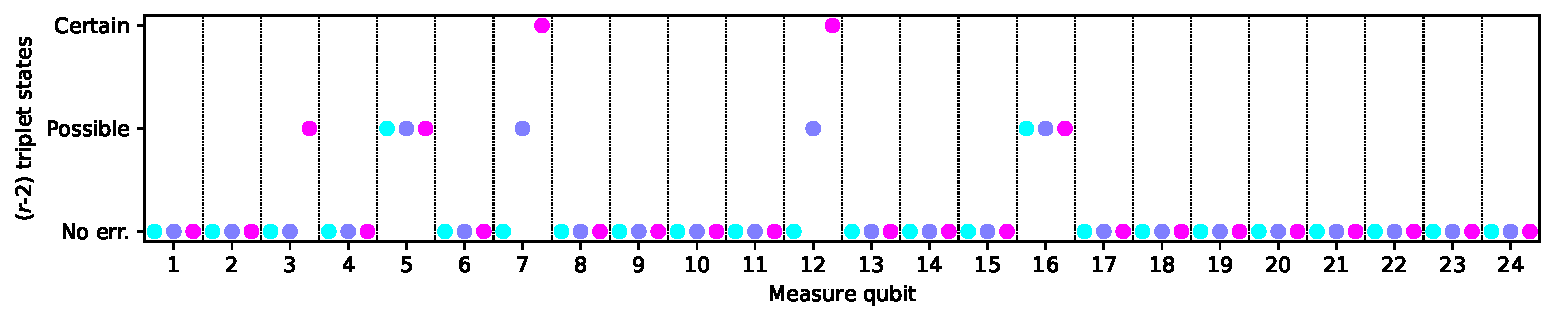
\includegraphics[width=0.9\textwidth]{states_d5_r5_event0.pdf} \\
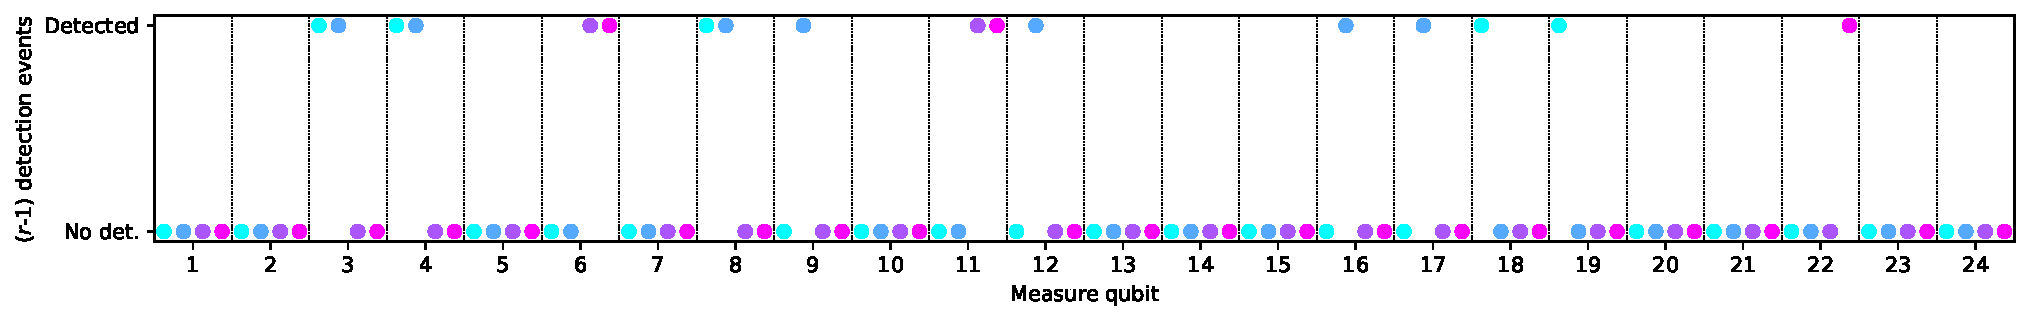
\includegraphics[width=0.9\textwidth]{det_evts_d5_r5_event0.pdf}
\ccaption
{Measure qubit raw states and detection events for $d=5$, $r=5$}
{
}
\label{fig:d5r5states}
\end{figure*}
%%%%%%%%%%%%%%%%%%%%%%%%%%%%%



\subsection{Recurrent convolutional kernel architecture for $r\geq 3$}
